\section{Plan de validation fonctionnelle}

Afin de vérifier le bon fonctionnement de notre programme, nous avons établi une stratégie de validation système. L'annexe \ref{APV} spécifie les tests de validation, l'organisation et la logistique de validation, ainsi que le plan documentaire. 

\section{Tests unitaires}

Enfin, des tests unitaires permettent de vérifier que chaque fonction est opérationnelle. Nous ne les détaillerons pas tous. Ainsi, nous nous concentrerons sur le critère 1.5.3 "Permettre le clic gauche / la sélection". Nous décrirons la procédure permettant de vérifier le bon fonctionnement d’une partie précise du logiciel, le click gauche. Nous testerons ce module, indépendamment du reste du programme, afin de nous assurer qu’il répond aux spécifications fonctionnelles et qu’il fonctionne correctement en toutes circonstances.
Notre projet comporte un fichier click.cpp où est implémentée la fonction
\begin{lstlisting}
bool closedEyesAndClick(cv::Mat faceROI, CascadeClassifier eyes_cascade)
\end{lstlisting}

Cette fonction permet à la fois de détecter si les yeux sont fermés ou ouverts et de cliquer. Elle fonctionne de la façon suivante (figure \ref{fig:CEAC}) :
\begin{itemize}[font=\tiny, label=\ding{108}]
\item Entrée :
\begin{itemize}[font=\tiny, label=\ding{109}]
\item Le premier argument est \lstinline=faceROI=, de type \lstinline=cv::Mat=. Cet argument est la matrice contenant l’image de l’œil.
\item Le second argument est \lstinline=eyes_cascade=, de type \lstinline=CascadeClassifier=. Cet argument est l’haar\_cascade permettant de détecter un œil.
\end{itemize}
\item  Sortie 1 : La sortie est \lstinline=yeuxFermes=, de type boolean. \lstinline=YeuxFermes= est à \lstinline=true= lorsque l’œil est fermé (pas de détection possible de l’œil) et à \lstinline=false= lorsque l’œil est ouvert. Cette sortie est utilisée par les autres modules de notre partie logicielle.
\item Sortie 2 : Une seconde sortie peut être considérée dans cette fonction, le clic qui agit sur l’OS.
\end{itemize}

\begin{figure}[H]
  \centering
  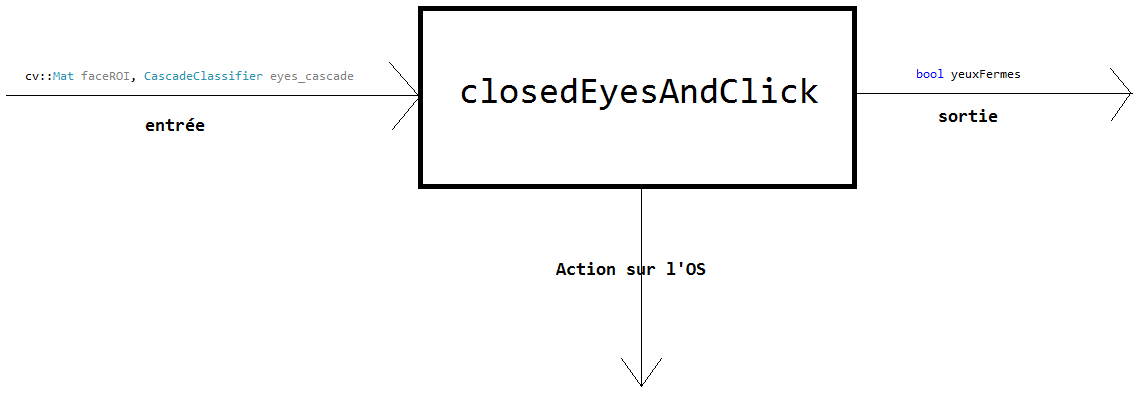
\includegraphics[scale=0.5]{fonctionClick}
  \caption{Fonction closedEyesAndClick}
  \label{fig:CEAC}
\end{figure}

Nous présenterons donc ici deux tests unitaires, le premier permettant de tester la détection de l’ouverture des yeux et le second permettant de vérifier l’action clic.

\subsection{Test Unitaire 1 : détection de l’ouverture de l’œil}

\paragraph{Les buts/attendus du test}

Le but du test est de vérifier que notre fonction renvoie bien le boolean \lstinline=true= lorsque l’œil est fermé et \lstinline=false= lorsque l’œil est ouvert. 

\paragraph{La préparation du test (mise en place, outils et instrumentation nécessaires)}

Nous avons codé un petit programme (voir annexe \ref{A1}) permettant d’acquérir un flux vidéo et d’appliquer notre fonction à ce flux. Une boucle \lstinline=while= permet, à chaque itération, de transformer l’image du flux en matrice \lstinline=cv::Mat=, de récupérer la sortie de la fonction et de l'afficher. De plus, nous avons fait en sorte qu’un rectangle soit tracé autour de l’œil lorsque celui est détecté, afin de mieux visualiser la détection ou non de l’œil.

\paragraph{Le déroulement du test}

\subparagraph{Conditions initiales (environnement) - Lancement du test}
L’utilisateur est assis à 50 cm de l’écran et de la webcam, positionnés face à lui. Le programme permettant d’effectuer le test unitaire est en cours de fonctionnement.

\subparagraph{Déroulement du test - Fin du test}

\begin{enumerate}
\item L’utilisateur garde les yeux ouverts. Nous vérifions que \lstinline=false= s’affiche dans le terminal et qu’un rectangle apparait bien sur l’image acquise par la webcam.
\item L’utilisateur ferme les yeux. Nous vérifions que \lstinline=true= s’affiche dans le terminal et que le rectangle ne s’affiche plus sur l’image acquise par la webcam.
\end{enumerate}

Ensuite, nous reprenons cette démarche avec l’utilisateur à 1 m de l’écran et de la webcam.

\paragraph{Analyse et consignation des résultats du test}

Après réalisation des tests, nous pouvons conclure que la méthode \lstinline=closedEyesAndClick= fonctionne correctement de 50 cm (comme nous pouvons le voir figure \ref{fig:OeilOuvert} et figure \ref{fig:OeilFerme}) à 1 m. En effet, de 50 cm à 1m, avec un pas de 10 cm, la fonction nous renvoie bien \lstinline=true= lorsque l’œil est fermé et renvoie \lstinline=false= lorsque l’œil est ouvert, tout en dessinant un rectangle autour de celui-ci.

\begin{figure}[H]
  \centering
  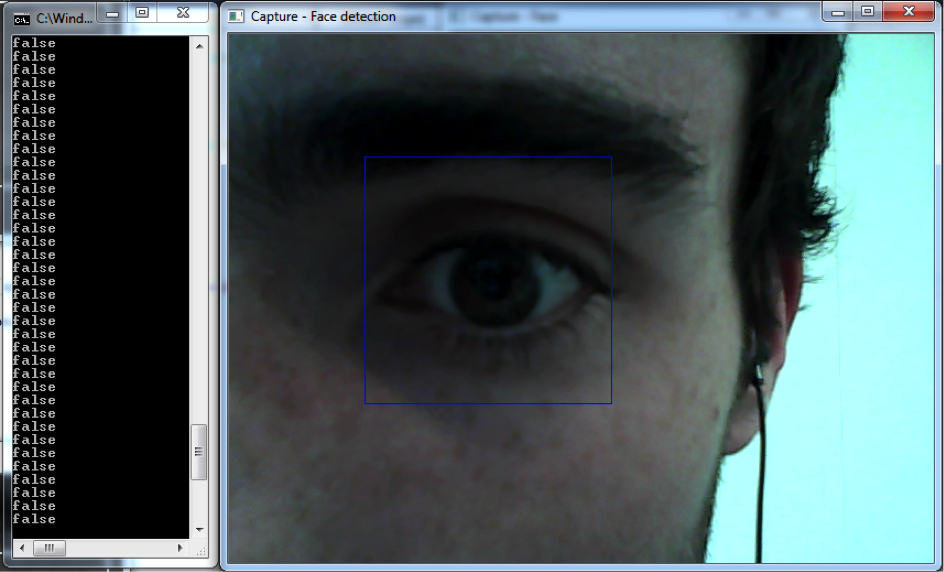
\includegraphics[scale=1]{OeilOuvert}
  \caption{Résultat du test unitaire pour la détection de l’ouverture de l’œil – Œil ouvert}
  \label{fig:OeilOuvert}
\end{figure}

\begin{figure}[H]
  \centering
  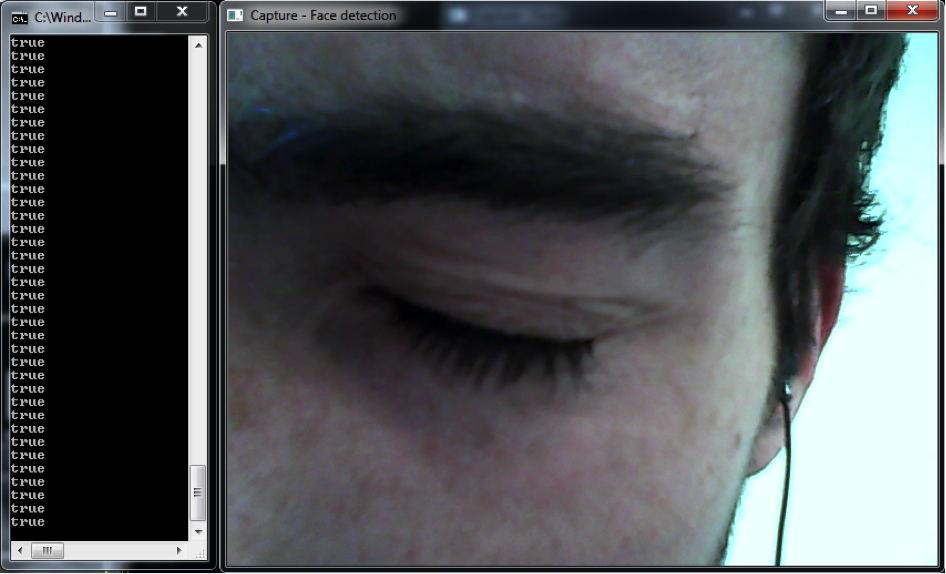
\includegraphics[scale=1]{OeilFerme}
  \caption{Résultat du test unitaire pour la détection de l’ouverture de l’œil – Œil fermé}
  \label{fig:OeilFerme}
\end{figure}

\subsection{Test Unitaire 2 : clic}

\paragraph{Les buts/attendus du test}

Le but du test est de vérifier que notre fonction permet le clic lorsque l’on ferme l’œil.

\paragraph{La préparation du test (mise en place, outils et instrumentation nécessaires)}

Pour préparer ce test unitaire, nous avons repris le programme du test unitaire précédant. Nous avons néanmoins ajouté la ligne \lstinline=printf("\a");= à la fonction \lstinline=closedEyesAndClick= afin de faire en sorte que l’ordinateur émette un bip lorsque le clic est déclenché.

\paragraph{Le déroulement du test}

\subparagraph{Conditions initiales (environnement) - Lancement du test}

L’utilisateur est assis à 50 cm de l’écran et de la webcam, positionnés face à lui. Le programme permettant d’effectuer le test unitaire est en cours de fonctionnement.

\subparagraph{Déroulement du test - Fin du test}

\begin{enumerate}
\item L’utilisateur garde les yeux ouverts. Nous vérifions que \lstinline=false= s’affiche dans le terminal et qu’un rectangle apparait bien sur l’image acquise pas la webcam.
\item Nous plaçons le curseur sur une fenêtre de l’OS se trouvant en arrière plan.
\item L’utilisateur ferme l’œil concerné par le test.
\item Nous vérifions que le rectangle disparait et que \lstinline=true= s’affiche dans le terminal.
\item Au bout de 1 seconde (minimum), l’utilisateur rouvre l’œil et nous vérifions que le bip sonore est bien émis et que la fenêtre sur laquelle se trouve le curseur passe au premier plan de l’OS. Nous constatons également que \lstinline=false= s’affiche dans le terminal et qu’un rectangle réapparait bien autour de l’œil.
\end{enumerate}

Ensuite, nous reprenons cette démarche avec l’utilisateur à 1 m de l’écran et de la webcam.

\paragraph{Analyse et consignation des résultats du test}

Après réalisation des tests, nous pouvons conclure que la méthode \lstinline=closedEyesAndClick= fonctionne correctement de 50 cm (comme nous pouvons le voir figure \ref{fig:OeilOuvert} et figure \ref{fig:OeilFerme}) à 1 m. En effet, de 50 cm à 1 m, avec un pas de 10 cm, le programme réagit comme prévu (passage de la fenêtre au premier plan).